\documentclass[../main.tex]{subfiles}

\begin{document}

In this chapter we introduce the main contribution of this thesis, we describe the proposed design flow and how it is implemented as part of the Halide infrastructure. 
In section \ref{motivations} we describe the motivations to use HLS tools to deploy DL models on FPGAs. We describe the main HW platform that can be used to perform inference and its drawbacks. 
In section \ref{back-end} we describe how the Bambu back-end works and how it is implemented inside the Halide infrastructure. We describe the main steps and possible future improvements.

\newpage

\section{Motivations}
\label {motivations}
Since the state of the art DL models are becoming increasingly more complex and demanding in terms of computational power, using CPUs and GPGPUs as inference platforms are becoming a less appealing approach. 
When a model is deployed the system is required to satisfy latency, throughput, and memory consumption constraints; CPUs are not suitable for high throughput applications, and power hungry GPUs have high latency due to memory transfers between host and accelerator.
The use of specialized ASICs meets all 3 requirements with high throughput, low latency, and memory consumption; but such a solution is not flexible and not able to express new layers that might have not been yet invented.

A different approach is to use Field Programmable Gate Arrays (FPGA); the use of programmable HW allows the possibility to satisfy all system requirements while being able to use the system to deploy different models.
The problem with FPGAs is the time required to deploy an FPGA's application; deploying a correct and optimized bitstream is not trivial and requires a long design time. To reduce that problem High-Level Synthesis tools are used; these tools take as input the abstract representation of a program, in this case, a DL model, and produce as output the optimized bitstream to be deployed. The final result does not have the same performance that a manually designed and optimized solution would have but allow fast prototyping and the use of FPGAs to deploy models without the need of being an expert in the design process.

The integration of a Bambu back-end in Halide allows the programmer to easily deploy a DL model on FPGA; the decoupling of the schedule from the algorithm definition allows the programmer to leverage the possibility to deploy multiple models in a short amount of time and find the schedule that better fit the target architecture and memory hierarchy.

\newpage

\section{Design flow}
\label {design-flow}
The goal of the proposed design flow is to leverage PandA - Bambu and the Halide infrastructure to deploy a Deep Learning model on FPGA while being able to optimize the sequence of scheduled operations for the target architecture.


\begin{figure}[h!]
  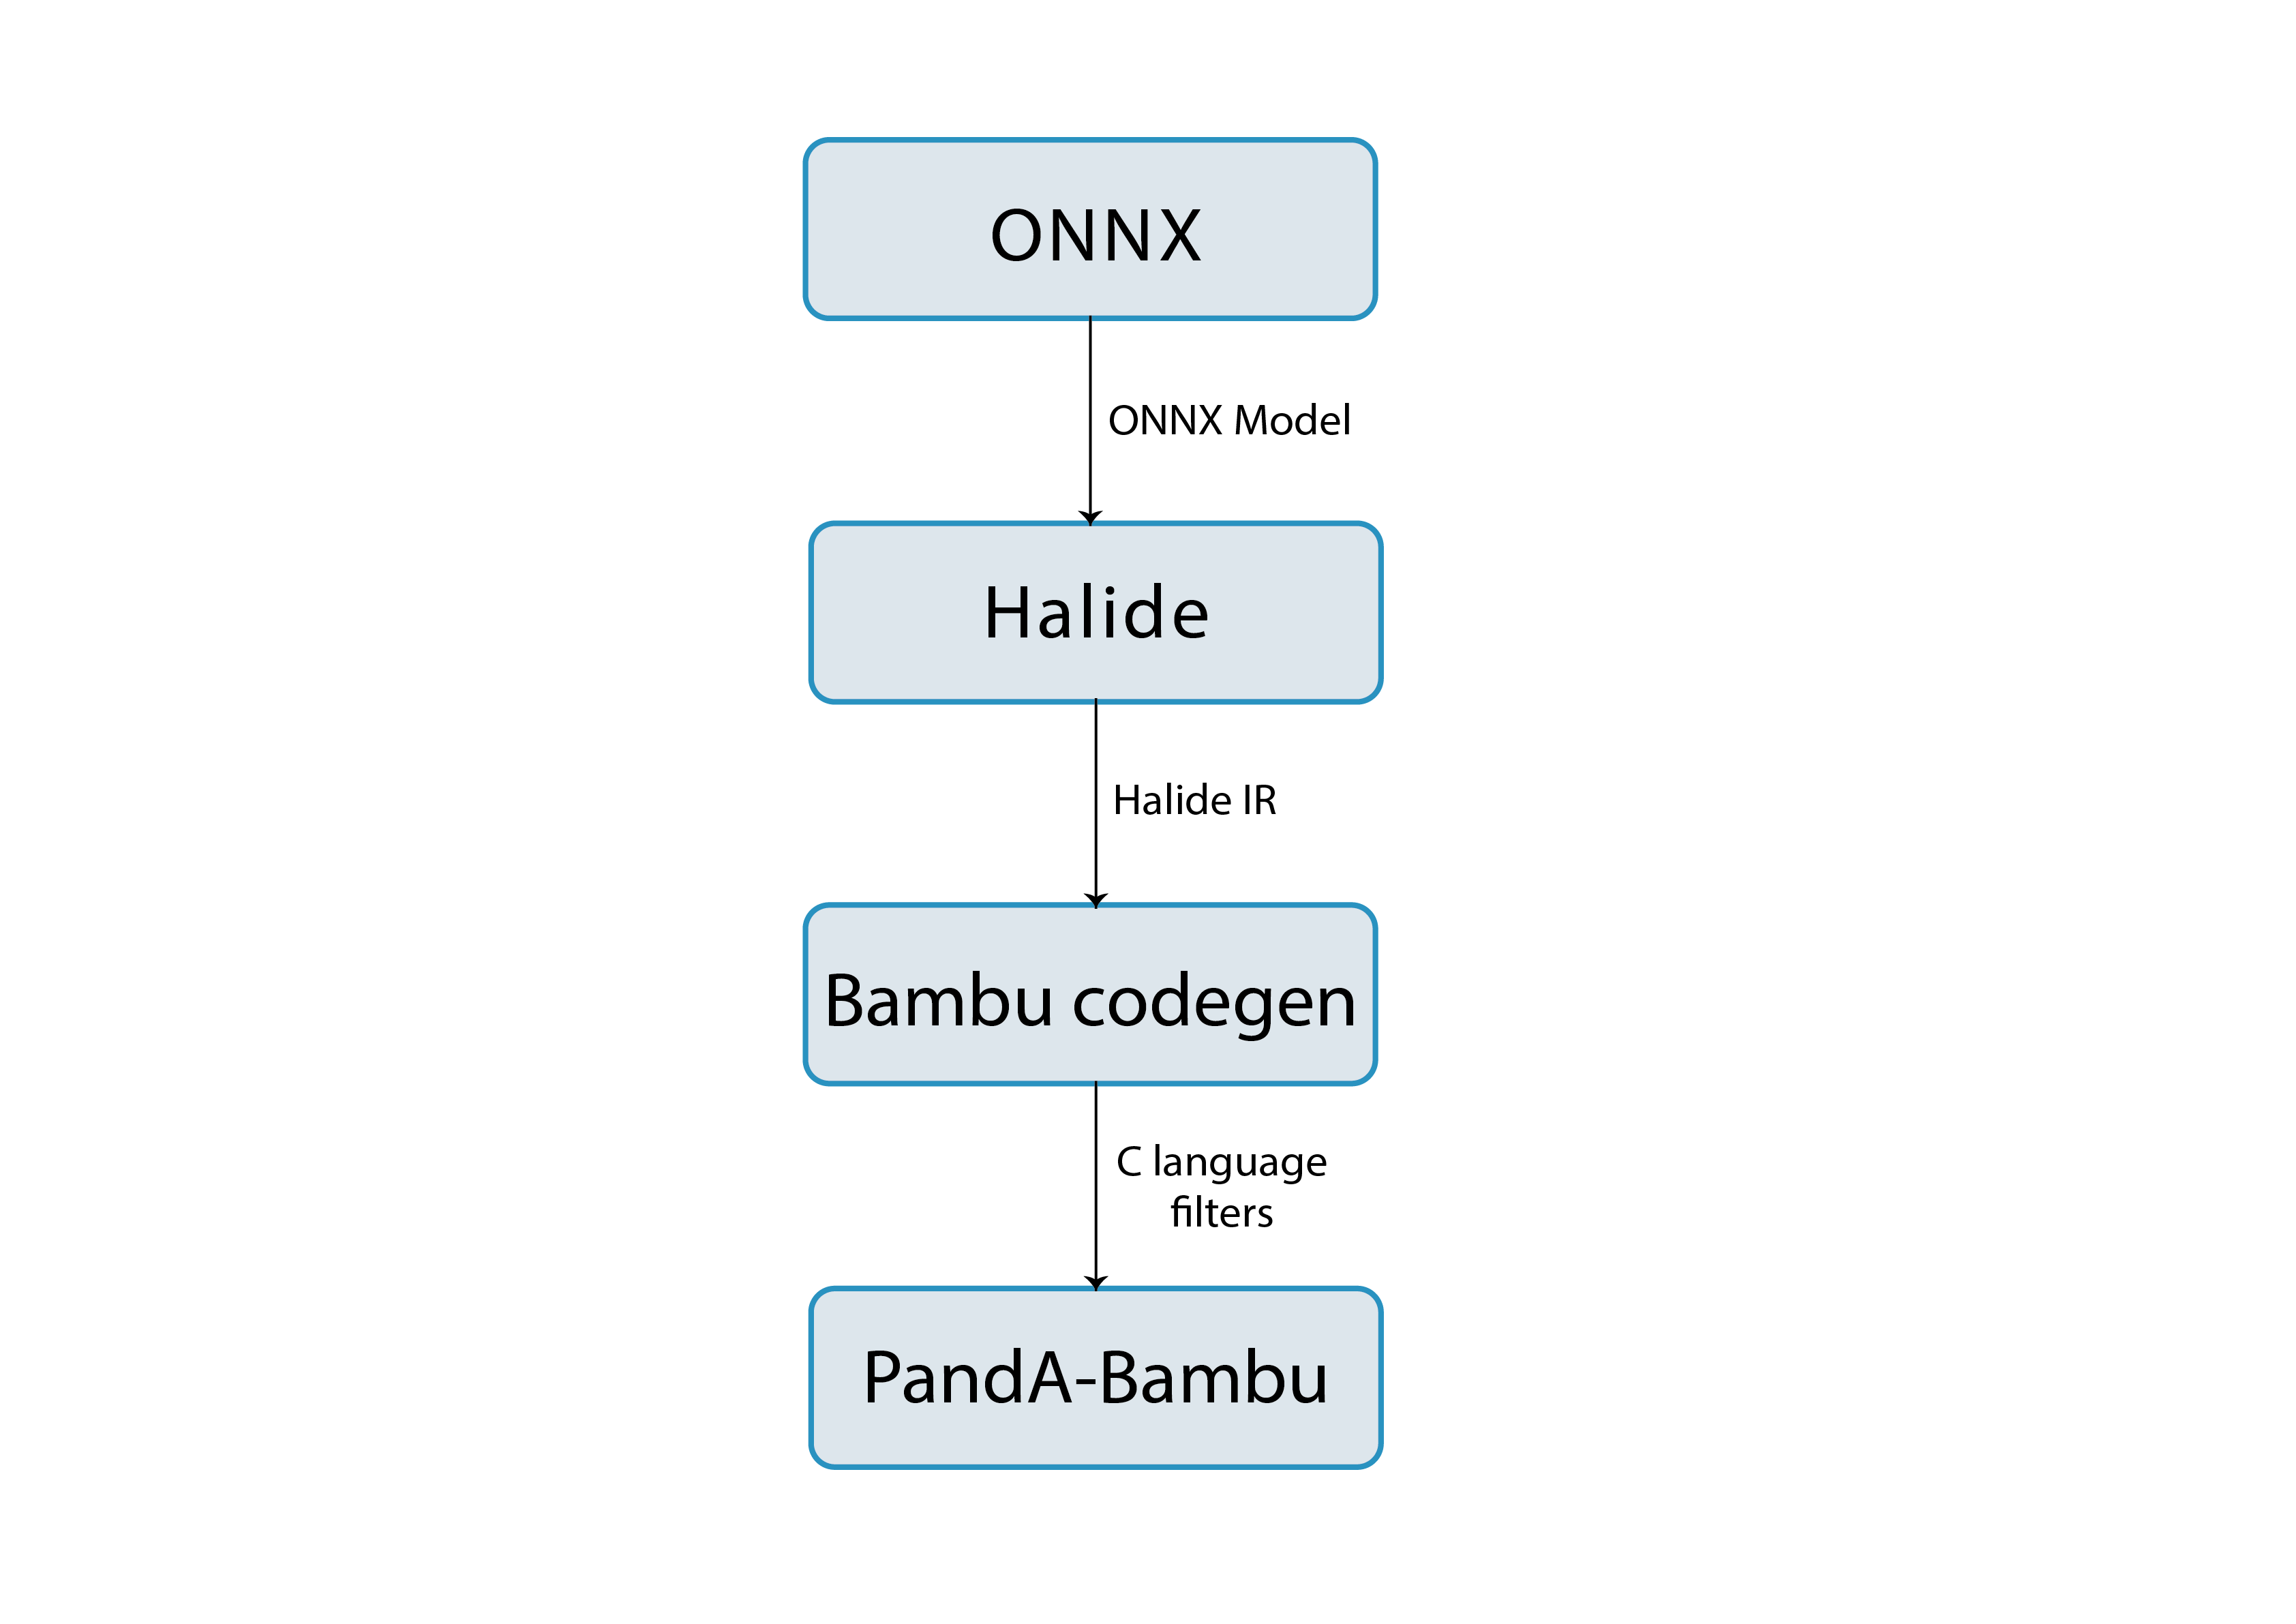
\includegraphics[width=1\textwidth]{images/Stack.png}
  \centering
  \caption{Design Flow}
  \label{fig:DesignFlowStack}
\end{figure}

\bigskip
The starting point is a Deep Neural Network model provided by one of the most common frameworks. Since each framework represents the computational graph in different ways we use a common representation to provide a unique entry point to the proposed design flow. The Open Neural Network eXchange specification (ONNX) has been used as a common representation; using ONNX allows the portability of computational graphs between different frameworks and is already supported by the Halide infrastructure.

To increase the performance of a forward pass of a DL model the design flow incorporates two optional steps: By using the VitisAI tools the programmer can perform pruning and quantization on the ONNX model. The pruning optimization increases the performance of the final model by reducing the amount of work that has to be done by removing the less useful connections between neurons and the quantization reduces the floating point precision of the operations. The latter is especially useful for FPGAs since the floating point precision can be easily adapted. 

Given the ONNX model that needs to be deployed the Halide framework has a built-in tool to convert it to an internal generator. The programmer can then decide how to schedule the imported model by defining the schedule method of the generator, as for any other algorithm. 

Halide can then proceed by converting the scheduled generator to an internal IR before feeding the optimized representation to the Bambu back-end that has been developed to provide support for FPGA targets.


\section{The Bambu back-end}
\label {back-end}
To implement a new back-end the Halide infrastructure allows the creation of target-specific codegens that take as input the Halide IR and produce the final optimized code. Each target architecture has its own back-end, that allows the Halide infrastructure to take advantage of architecture-specific features and optimizations.

The Bambu back-end takes as input the Halide IR and produces the C code to be used within the Bambu framework. The code generation is split into 3 main steps: Filter extraction, IR optimizations, and code generation. The next sections describe the three steps in detail.

\subsection{Filters extraction}

The filters extraction step takes as input the Halide IR and produces a DAG representation of the Halide lowered function. 
The DAG is composed of interconnected filters related to a producer-consumer relationship. 
Such a relationship is already extracted by the Halide infrastructure and can be easily extracted by leveraging the ProducerConsumer statement of the Halide IR.

Before proceeding with the extraction of the DAG filters the codegen prepare the Halide IR by preprocessing filters and buffer names.
The ONNX model already specifies these names and the Halide IR does not check if the name starts with a number and if special characters are present.
Moreover, the Halide IR does not check for clashing buffers and filters names.
The codegen changes these names by substituting special characters with an underscore and by renaming buffers and filters by adding a unique identifier at the end.

After the preprocessing step of the ONNX identifiers, the next is the substitution of available compile-time information.
The Halide IR consider the sizes of input and output tensors as data that are known only during runtime execution and retrieve such information when the input and output tensors are passed to the function.
Since the ONNX model does not work as a general image processing pipeline, the information about input and output tensors is fixed and already present inside the ONNX representation.
We can then take the values already present in the ONNX model and substitute them inside the Halide IR; this step simplifies the loop extents generated by the Halide's bound inference procedure, usually leading to loops with a constant extent.

With the unique identifiers set and the compile-time information provided by the ONNX model already incorporated inside the Halide IR, the next step is to eliminate constructs not necessary for the extraction of the DAG representation.
Since the Halide IR retrieves information about the input and output tensors at runtime, the generated IR performs a sequence of checks on the input data before starting the computation.
These checks involve detecting if the extends are negative and if the input tensors have the sizes different than the ones specified by the ONNX models.
These checks are useless for the translation of the Halide IR and are therefore removed.

The last step before translating the Halide IR to a DAG representation between filter is the simplification of the IR.
The Let statements inside the IR code are eliminated and substituted inside other constructs; this will turn useful during the IR optimization when we will push as outside as possible all stores that do not depend on the inner loop variable.
Since the names of loop variables are complicated and contain several special characters they are substituted with new and unique identifiers; variable names inside the IR are substituted accordingly with the unique identifiers assigned to the corresponding loop.

\begin{lstlisting}[caption= Example of filter extracted from the Halide IR. The extracted code is hard to translate to c language and access the memory buffers at each iteration. ]
X_im_padded_U_sum_3[0] = 0.000000f
for (x_7, 0, 3) {
    for (x_8, 0, 3) {
        X_im_padded_U_sum_3[0] = ((float32)X_im_padded_U_sum_3[0] 
          + ((float32)b2[((x_7*6) x_3)]
          * ((float32)b2[((x_8*6) + x_4)]
          * (float32)b0[((((x_2*3) + x_8)*3) + x_7)])))
    }
}
\end{lstlisting}

Another important simplification is about Allocate statements.
Since the allocation of buffers with constant size is important to produce an efficient result; nonconstant buffer sizes are substituted with the maximum possible size allocated during execution.
To do so the codegen considers the expression corresponding to the allocated size and by considering the minimum and maximum values of all contained variables find and substitute the maximum allocated size of the buffer.


With the input IR containing all the available compile-time information and cleared of unused constructs, we are ready to translate the preprocessed IR to a DAG representation.
The first step is the extraction of the Stages already extracted by the Halide IR.
The stages are already represented ad Producer-Consumer relationships, the codegen uses these relationships and extract one stage for each producer element in the IR.
The elements extracted are then connected according to Producer-Consumer relationships present in the IR.
To extract the relationships when a consumer statement is found a Producer-Consumer relationship is created between the consumed stage and the innermost producer.

When all stages have been extracted with all the Producer-Consumer relationships the codegen is ready to create the DAG representation among filters.
Since it is easier for Bambu HLS to parallelize function calls instead of entire bodies of for loops we decided to split the stage code into multiple functions.
To do that when the code contains loops marked as parallel the codegen split the stage into multiple filters.
The result is a collection of filters connected by function calls; when a loop is meant to be parallelized the body of the loop always contains only one function call to the function intended to be executed in parallel.

Since the Halide schedule allows the execution of multiple stages at root granularity, the DAG obtained by the previous steps might have multiple filters that are not invoked by others.
This introduces the necessity of having a unique entry point that executes these filters in the order specified by the Halide IR.
To finalize the extracted DAG before proceeding with the optimization phase we need to introduce one additional filter meant to be used as the entry point of the computation.
The codegen introduces a filter named "bambu\_main\_filter"; the new filter allocates the necessary buffers and invokes the functions executed at root granularity in the order specified by the Halide IR.


\subsection{IR optimizations}

Once the filters have been extracted, the program has been represented as a set of interconnected independent filters related to producer-consumer relationships.
Each filter has its independent code represented as a Halide statement and the IR code must be optimized by performing a set of optimization passes over the IR code representation, such as reducing as much as possible redundant memory accesses and by avoiding recomputation of data shared by different iterations.

The first step is to extract the necessary information by visiting the IR code.
The set of variables and buffers accessed during the code execution are stored with their required data type, and if they are not allocated inside the IR code, they are marked as parameters of the filter.
Dependencies between filters are extracted from the function calls generated by the stage to DAG translation, and the information about allocated buffers is stored in a map common to all filters containing the type and the size of the buffer as an expression of other variables.

A second important piece of data collected from the code IR is the kind of access performed by the filter on a specific buffer.
A filter can access a buffer by reading the content of the buffer with a Load statement or by saving something on the buffer by accessing it with a store statement.
The codegen collects information about the filters accessed during execution, the type of access performed, and if they are accessed multiple times.

Once the necessary information is extracted from the IR of the filter the codegen must prepare the IR for the optimization passes.
The IR is currently stored as a loop nest containing all the operations in one store statement in the innermost loop; this happens because in a preprocessing step we decided to remove all let statements by substituting them into the cleaned IR.
This has been done to reduce the number of parameters required by a filter but the resulting IR is not suitable to be used as a starting point.
To prepare the IR for the optimizations we decided to split the store statements in multiple elementary stores that perform one operation before assigning the result to a unique variable.
This is done by recursively producing a store statement for each operator, each store computes one elementary operation and stores the result in an intermediate variable.
While doing that, the codegen check if the operator to be produced is already computed and stored in another variable.
If that happens the codegen avoids recomputing the result and uses the already computed value.

Now that the necessary data have been retrieved and the IR has been preprocessed the IR is ready to be optimized.
The first optimization step that is performed on the preprocessed IR is pushing as outside as possible each store statement while preserving the order of computation of operators that depend on the same set of variables.
To do that, firstly, the codegen needs to compute the dependency of each store statement to each allocated variable inside the filter's IR; this information is then leveraged to push as outside as possible each store statement.
The codegen check at every declaration if the newly declared variable satisfies the requirement of some of the store statements that still need to be placed inside the mutated IR code; if for some variable that happens, the codegen moves the store operation after the new declaration.
If multiple declarations have all dependencies satisfied by the new declaration the codegen places the store statements without altering their relative order.

\begin{lstlisting}[caption = Example of optimized IR. The complex operation of the previous example has been split into simple operations. Intermediate results that are shared among different iterations and memory accesses has been pushed outside]
X_im_padded_U_sum_3[0] = 0.000000f
_9[0] = (x_2*3)
_17[0] = (float32)X_im_padded_U_sum_3[0]
for (x_7, 0, 3) {
    _3[0] = (x_7*6)
    _4[0] = (_3 + x_3)
    for (x_8, 0, 3) {
        _6[0] = (x_8*6)
        _7[0] = (_6 + x_4)
        _10[0] = (_9 + x_8)
        _11[0] = (_10*3)
        _12[0] = (_11 + x_7)
        _2[0] = (float32)_17
        _5[0] = (float32)b2[_4]
        _8[0] = (float32)b2[_7]
        _13[0] = (float32)b0[_12]
        _14[0] = ((float32)_8*(float32)_13)
        _15[0] = ((float32)_5*(float32)_14)
        _16[0] = ((float32)_2 + (float32)_15)
        _17[0] = (float32)_16
    }
}
\end{lstlisting}

The previous optimization cannot be performed on store and load operations on buffers.
Some operations produced by the Halide infrastructure are intended to be performed multiple times on the same index and pushing outside these operations would affect the correctness of the final program.
Pairs of load and store operations on the same buffer and at the same index can be optimized by performing the memory access as outside as possible in the loop nest.
The computation can then be performed on a local variable before storing the final result only at the end of the computation.
To perform the optimization on the filter's IR the codegen detect, for each loop, when an inner pair of load and store operations do not depend on other variables.
If that happens, the codegen load the current buffer value in a local variable, substitute the load and store operations inside the loop body with the newly declared temporary variable and store back the computed result at the end of the loop body.

Another important optimization step is the detection of queues between filters. 
The Bambu framework can implement FIFO connections as communication mechanisms between filters and the codegen can optimize the IR by detecting when a pair of load and store statements need to be substituted with dequeue and enqueue operations.
The current implementation of this optimization considers for each filter its output connections.
Before checking if the indexes of the two operations match the connection must satisfy some preliminary constraints.
For each considered connection, the starting and ending filters must have correspondingly one write and one read operations on the considered buffer.
Moreover, the two operations must be parallelized under the same variables and have a matching loop nest.
If all the prerequisites are satisfied, the codegen can compare the indexes of the two operations, and if they match the store and load operations are substituted with dequeue and enqueue operations.


\subsection{Code generation}


Before producing the final code the generation phase needs some preprocessing.
When we extracted the information about the buffers and the variables we detected the required arguments by identifying the ones that are not declared by the filter.
This mark correctly buffers and variables that need to be allocated elsewhere as parameters but there is no guarantee that they are going to be available to the invoking filter.
Some parameters might be allocated in a different filter connected through multiple sequential connections in the DAG.
For that reason, as preprocessing step, we need to propagate the parameters until they reach the declaring filter.
The codegen iteratively considers the parameters required by the filter invocations; if they are not declared they are added as requested parameters to the caller of the filter.
The step is repeated until the requested parameters reach a fixed point.

After the parameters have been propagated the next preprocessing step is to finalize the function calls.
Until that point, each call has been represented by only the name of the filter that needs to be called; now that the parameters are available we can change the function call with the actual signature of the function.

Store and load operations on buffers can also be finalized;  read operations on queues are changed with dequeue operations.
Conversely, since store operations may write on multiple queues while also writing on an array buffer, the codegen generates the necessary enqueue and write operations.

Once the IR has been preprocessed the codegen is ready to produce the final C filters.
After the inclusion of the necessary dependencies, like prototypes for invocations and vectorized operations, the codegen produces the function signature by using the data collected about the return value and the required parameters.
The filter's IR is then translated to a valid C code by translating line by line the IR representation.
The final code is produced by encapsulating the translation line by line of the IR in the previously created function signature.

To avoid declaring multiple times the same variable, the codegen keeps in memory the name of previous declarations.
Therefore, if a store operation assigns a result to an already declared variable the codegen generates the assignment without declaring the LHS variable.

\begin{lstlisting}[caption = Output C code of the example filter. The Halide IR has been translated to C code and encapsulated. Since the filter compute only one value a return statement has been added at the end of the function.]
float X_im_padded_U_sum_3_fun_0(float b0[18], float b2[18],
        int x_2, int x_3, int x_4){
    float X_im_padded_U_sum_3 = 0x0p+0;
    X_im_padded_U_sum_3 = 0x0p+0;
    int32_t _9 = x_2 * 3;
    float _17 = X_im_padded_U_sum_3;
    for(unsigned int x_7 = (0); x_7 < (0 + 3); x_7++){
        int32_t _3 = x_7 * 6;
        int32_t _4 = _3 + x_3;
        for(unsigned int x_8 = (0); x_8 < (0 + 3); x_8++){
            int32_t _6 = x_8 * 6;
            int32_t _7 = _6 + x_4;
            int32_t _10 = _9 + x_8;
            int32_t _11 = _10 * 3;
            int32_t _12 = _11 + x_7;
            float _2 = _17;
            float _5 = b2[_4];
            float _8 = b2[_7];
            float _13 = b0[_12];
            float _14 = _8 * _13;
            float _15 = _5 * _14;
            float _16 = _2 + _15;
            _17 = _16;
        }
    }
    X_im_padded_U_sum_3 = _17;
    return X_im_padded_U_sum_3;
}
\end{lstlisting}

Since some operations can not be specified inside the Halide IR, the codegen implement other optimizations during the code generation phase.
When a filter implements an add bias operation the output code is composed as a sequence of if operators, which is highly inefficient.
The codegen optimizes such operation by storing the values in a static array and by accessing the right one by index.

Another optimization is the optimization of ramp operations on vectorized operations.
When the values of the ramp operation are known at compile-time, the codegen can directly allocate the ramp values without computing them at runtime.
This is done by statically allocating the array containing the ramp values.

\section{Parallel and vectorized operations}
An important factor that influences the performance of the schedule on the target architecture is how to handle coarse and fine-grained parallelism.
In the halide infrastructure, coarse-grained parallelism is represented by parallel loops that represent pieces of computation that can be performed independently without modifying the correctness of the output buffers.
Fine-grained parallelism is represented by vectorized operations on vectors.

To handle coarse-grained parallelism PandA-Bambu allows the definition of for loops parallelized with the \#pragma omp for directive. This allows to perform each independent iteration in parallel and on different HW resources.

\bigskip
\begin{lstlisting}[caption = Example of coarse-grained parallelism exploited by parallelizing independent iterations. The final model will perform each iteration of the for loop on different resources.]
    #pragma omp for
    for(unsigned int x_0 = (0); x_0 < (0 + 53); x_0++){
        _conv1_2_0_fun_0(b0, conv1_2_0, b1, data_0, x_0);
    }
\end{lstlisting}

\bigskip
Fine-grained parallelism is handled by performing vectorized operations on small arrays. The usage of vectorized operations on simple independent operations allows to exploit the advantage of FPGA platforms on fine-grained operations.

\bigskip
\begin{lstlisting}[caption = Example of vector multiplication exploiting vectorized operations. In this example the multiply operation is performed on small arrays representing vectors of 8 elements.]
void _Z_fun_0(float X_im_0[8], float Y_im_1[8], float Z[8]){
    int32_t _0[8] = {0, 1, 2, 3, 4, 5, 6, 7};
    float _1[8];
    load_vector<float, int32_t, 8>(_1, X_im_0, _0);
    float _2[8];
    load_vector<float, int32_t, 8>(_2, Y_im_1, _0);
    float _3[8];
    binary_op<float, float, 8, std::multiplies<float>>(_3, _1, _2);
    store_vector<float, int32_t, 8>(Z, _3, _0);
}
\end{lstlisting}

\newpage
\section{Additional generated code and files}

When the codegen has produced all the necessary filters to perform the computation, we still need some additional code and files.

To be able to start the computation, the generated C filters require the definition of multiple static buffers.
These buffers are generated by the Halide infrastructure; they are represented as arrays of data that do not change during the computation and are necessary to compute the correct result.
In our case, since we are considering ONNX models, these buffers usually contain the weights of the Deep Learning model; without them, the application would not be able to compute the correct transformation of the input tensor.

To ease the loading procedure of these buffers, we decided to store them into dedicated .dat files.
The programmer can use a handle function to load each buffer into memory without the need to know how the data are organized.
Moreover, this allows the programmer to easily swap the buffer values by loading different ones, without the need to recompile the entire ONNX model.

Another file produced is the one containing handle functions for vectorized operations, named Vectorization.hpp.
When vectorized operations are produced, the filter uses small arrays to store the vectors.
Instead of writing each operation every time as a parallel loop over the elements of the array, the filter calls a handle operation that performs the computation on the vectors.
This makes the code easier to read and reduce the size of the generated filters.

\section{Conclusions}
In this section we described the structure of the design flow. We described the steps necessary to optimize and deploy a DL models using the ONNX representation, the Halide infrastructure, and PandA-Bambu as HLS tool. We described how is the Halide Bambu codegen structured and how it works.



\end{document}